\section{Background and motivation}
\label{ch-introduction:sec:background}

Today's society and economy are highly dependent on the continuous availability of energy or more specifically: electric energy.
In the UK, demand for electricity has increased over the past decades, and this trend is expected to continue into the future \cite{HMGovernment2009}.
This demand increase is only accelerated since a major focus of UK energy policies has been put on transitioning towards a low carbon economy \cite{RoyalAcademyofEngineering2010}.
Particularly the decarbonisation of heat and transport sectors are two areas of significant strategic focus and Low Carbon Technology (LCT) such as Photovoltaic (PV) installations, Electric Vehicles (EVs) and heat pumps are expected to contribute significantly to the energy mix of this transition.

\nomenclature[G]{FES}{Future Energy Scenarios}

As uptake of these LCTs continues and they start penetrating power distribution networks, stress on these networks will also continue to increase, resulting in operating issues that can eventually lead to additional service disruptions.
Furthermore, the uptake of LCTs is not expected to progress evenly throughout the entire power network, but instead clusters of early adopters are predicted to form, leading to certain LV networks exceeding their operational constraints even at a relatively low national rate of LCT adaption \cite{Poghosyan2014}.
The scale of this energy transition becomes becomes particularly apparent when referring to the UK's 2017 Future Energy Scenarios (FES) that compare the predicted future load scenarios for the upcoming decades \cite{FES2017}.

\begin{figure}\centering
	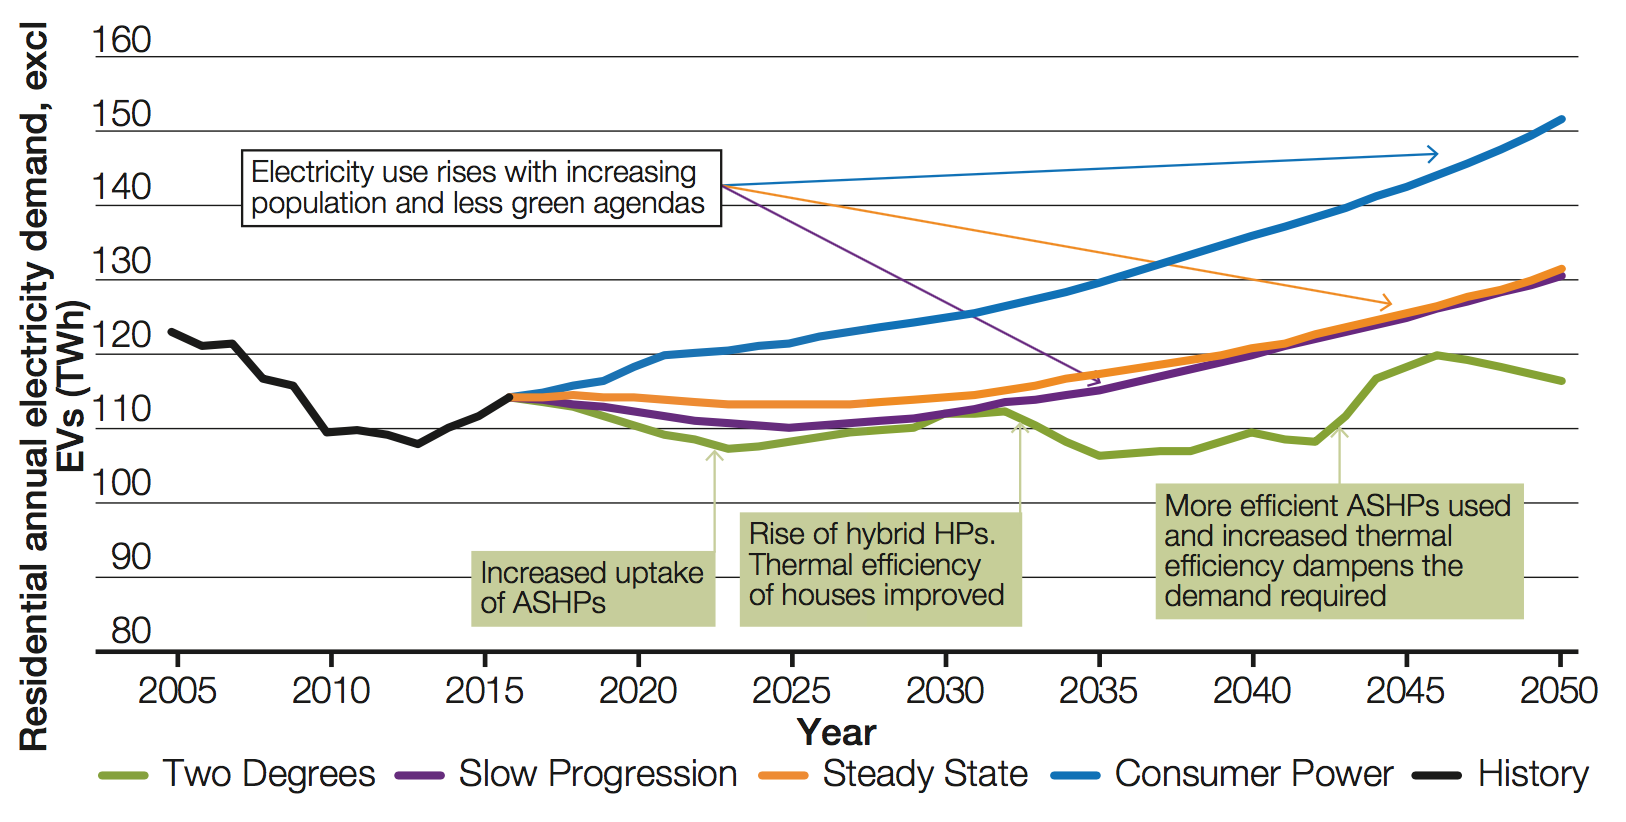
\includegraphics{_introduction/fig/electricity-demand-residential}
	\caption{Change in residential annual electricity demand excluding electric vehicles from FES2017 \cite{FES2017}}
	\label{ch-introduction:fig:electricity-demand-residential}
\end{figure}

Figure~\ref{ch-introduction:fig:electricity-demand-residential} shows the predicted increase in annual residential electricity demand; here the market driven scenario (i.e. ``Consumer Power'') shows the largest increase until 2050.
When putting more emphasis on environmental concerns, the ``Two Degrees`` scenario emerges.
This scenario refers to the intention of limiting global temperature increase to two degrees (previous FES reports referred to this scenario as ``Gone Green``).
According to the FES 2017 those two scenarios enable a continuing growth of the UK economy, but put very different emphasis on decarbonisation targets.
Although the rise in demand for electricity is projected to differ by more than 30TWh in 2050 (i.e. if the ``Two Degrees`` scenario is achieved), the aforementioned uptake of LCTs like EVs is expected to put additional load onto the power network in both scenarios.

\begin{figure}\centering
	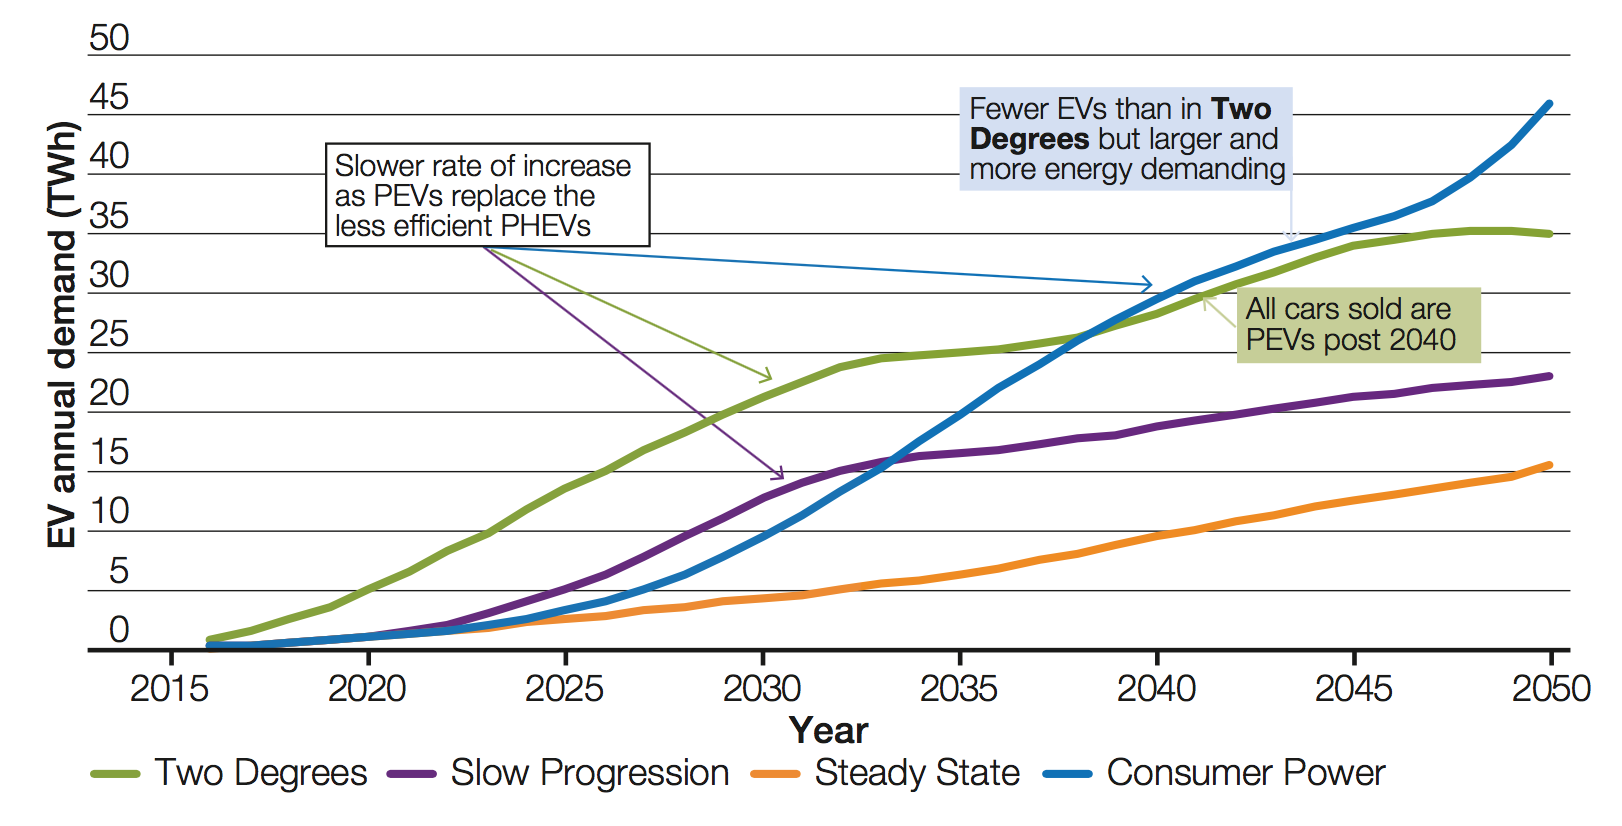
\includegraphics{_introduction/fig/electricity-demand-ev}
	\caption{Rise in energy demand due to the uptake of electric vehicles as predicted by FES 2017 \cite{FES2017}}
	\label{ch-introduction:fig:electricity-demand-ev}
\end{figure}

When focusing on the electrification of personal transport (by introducing EVs into the electricity demand), Figure~\ref{ch-introduction:fig:electricity-demand-ev} shows that both the ``Consumer Power'' as well as the ``Two Degrees'' scenario will add more than 35TWh of annual energy demand by 2045.
Since most of these EVs are expected to charge at home and (at least initially) at similar times, aggregating effects are feared to not only exhaust national energy supply capabilities but also power distribution capacities.

\begin{figure}\centering
	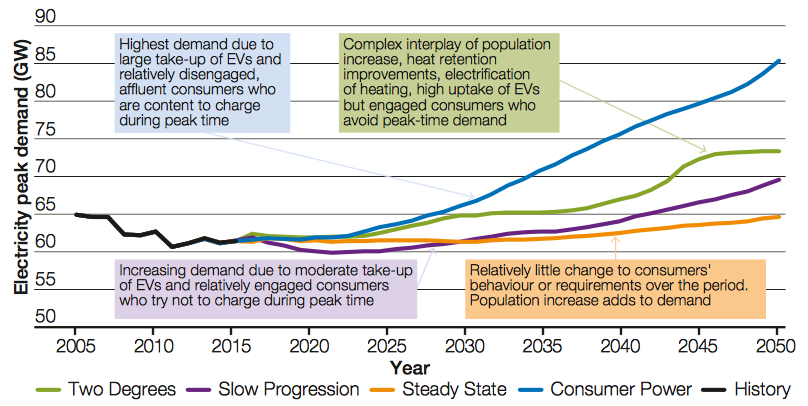
\includegraphics{_introduction/fig/electricity-peak-demand}
	\caption{Change in annual peak power demand as predicted by FES2017 \cite{FES2017}}
	\label{ch-introduction:fig:electricity-peak-demand}
\end{figure}

\nomenclature[G]{CREST}{Centre for Renewable Energy Systems Technology}
\nomenclature[G]{ENW}{Electricity North West}

Figure~\ref{ch-introduction:fig:electricity-peak-demand} supports this fear since uncontrolled proliferation of LCTs and EVs (as shown in the ``Consumer Power'' scenario) will add more than 20GW of power demand onto today's peak power levels.
Such a rise in peak power would exceed today's supply capacities, especially since the new energy mix and decommissioning of fossil fuelled power plants have resulted in this year's winter capacity margin to only lie between 3.7GW and 4.9GW \cite{NationalGrid2017a} (this equates to a 7.2\% margin whilst in for example 2010 this margin was at 15\% with 11.7GW \cite{NationalGrid2010}).

Although FES 2017 expects the ``Two Degrees'' scenario to also show an increase in peak power, better coordination and control is expected to mitigate half of the 20GW peak increase.
From this point of view, today's narrow capacity margins could already cater for nearly half of the increase in peak demand that is expected to occur over the next 33 years (i.e. until 2050).
Whilst UK power transmission networks are being upgraded and will therefore be capable of handling this increased power demand, the increasing stress on the distribution network still remains.
This stress is due to the fact that loads in the residential and commercial sectors are typically situated at the network edge (i.e. in the LV distribution network) and reinforcing these networks can result in costly service disruptions.

\subsection{Topology and challenges of the UK electricity network}
\label{ch-introduction:subsec:topology-of-lv-network}

The UK electricity network in today's form has grown over the past century and is based on an interconnected high-voltage network.
Its largest part is also known as the transmission network, which connects remote power stations to distribution networks.
Typically those distribution networks supply electricity to all loads across the mainland of the UK, including industrial, urban and rural customers\footnote{Some small and remote UK islands like the Shetland islands are not connected to this national grid and have their separate electricity infrastructure. Therefore they are not considered as part of this thesis since the study of this kind of network lies outside the research scope.}. For instance, larger customers that are not situated within the distribution network need not be supplied by said network.

The entire structure of the electricity network is a three-phase Alternating Current (AC) system since this allows easy voltage level conversion with the use of transformers, i.e. without the need for power electronics.
In the UK, the highest voltage level for generation and transmission is 400kV.
Such a high voltage requires a relatively small current to transmit the generated bulk power, which in turn reduces conduction losses and maximises the efficiency of the high-voltage network.
Regional supply points step-down this high voltage to 132kV\footnote{In some cases regional supply points provide 127kV instead of 132kV.} to deliver power to Distribution Network Operators (DNOs).
From the primary level of the distribution network and onwards, this so called medium-voltage is stepped down to 33kV, then 11kV and finally 400V phase to phase (P2P), in order to cater for heavy industry, medium clients and household sized customers, respectively.
In the UK, all households are connected to one of the three phases of the distribution network and therefore are supplied at a nominal voltage of 230V (phase to neutral - P2N).
To achieve a balanced network, each customer's phase allocation is chosen at pseudo-random\footnote{Guidance for customer phase allocation is not explicitly specified in the network's design framework~\cite{UKPowerNetworks2014}. Therefore, choosing the ``top phase'' qualifies as pseudo-random phase allocation with statutory compliance~\cite{StatutoryInstruments2015}.}.

\nomenclature[G]{DER}{Distributed Energy Resource}
\nomenclature[G]{ADMD}{After Diversity Maximum Demand}
\nomenclature[G]{OLTC}{On-Line Tap-Changer}

This LV part of the electricity network is its weakest part, since its assets were designed to cater for small powers between 315kVA to 500kVA \cite{EDS08-0115}.
Despite this capacity limitation, DNOs aim to maintain distribution level voltages within their statutory operating bands, i.e. 230V +10\% -6\% for the LV network as specified by the Electricity Supply Quality and Continuity Regulation (ESQRC) \cite{HealthandSafetyExecutive2002} and Engineering Recommendation G59 \cite{EnergyNetworksAssociation2013}.
Primary substations in the UK are equipped with regulation equipment, like On-Line Tap-Changers (OLTC), to increase or decrease the voltage on the secondary transformer side depending on the current level of demand.
Secondary transformers do not have such regulating equipment and instead apply a constant voltage conversion ratio which is set according to the network's typical demand.

A project based on the findings from \textit{Electricity North West} (ENW) in \cite{ElectricityNorthWestLtd2014} emphasises the issues that result from residential increase in demand for electricity; like voltage deviation due to an uptake of LCTs.
More specifically, in the ENW lead project 200 LV networks in the UK were monitored to assess the capacity for LCT adoption.
Initial findings showed that even in today's distribution networks, 15\% of all monitored substations experienced reverse power flow, 4.5\% substations reported high voltages (i.e. above 253V), and only 2\% substations reported occasional low voltages (i.e. below 216V).
With the voltage drop assumption however, it was believed that customers in these network were still operating at BSEN50160 compliant voltage levels.
Models to assess the LCT headroom indicated that the first issue is always voltage deviation and thermal or capacity limits are of second concern.
This finding is based on the fact that LV networks are highly resistive and rarely managed in an active manner; hence as the number of PV installations is expected to grow the voltage deviation magnitude and frequency is also going to increase \cite{Woyte2006}.
Since the expected voltage deviation was caused despite a relatively low adaptation of residential LCTs, strict precautionary regulation has been put in place to assure continuous operation without violating any operating constraints.
Otherwise additional voltage deviation, unbalanced network operation or asset overloads could be the result.

Traditional network planning approaches that have been used by DNOs to expand and install network assets were designed to circumvent such issues in order to follow the aforementioned standards and regulations.
The most common approach follows the commonly used practice of aggregating a large number of customers and designing the power delivery network to cater for their largest probable demand, i.e. the After Diversity Maximum Demand (ADMD) method \cite{Richardson2010a}.
This ADMD method has remained the same for many years and uses historical load analysis and standard growth assumptions that are both no longer valid in this unprecedented LCT uptake scenario \cite{Yunusov2016}.
To make things worse, LV networks in the UK are generally unmonitored once installed \cite{Yunusov2016}.
Distribution Network Operators (DNOs) have become aware of this issue and are developing updated planning strategies involving ``smart'' and ``flexible'' electricity grids \cite{Fang2012}.
However, in situ equipment that will become subject to the same adaptation of LCT needs to be managed actively via innovation in the use of existing and new technologies; otherwise both frequency of service disruptions and customer minutes lost will increase alongside the proliferation of LCTs \cite{Ault2008a}.
One such innovative technology, which is the main focus of the presented thesis, is the installation and management of battery storage \cite{Chen2009}.
The following section is going to introduce the two favoured solutions to address network issues and explain why battery energy storage was chosen as part of the presented research.


\subsection{Solutions to mitigate impact of LCT}
\label{ch-introduction:subsec:solutions-to-mitigate-impact-of-lct}

The two most favoured solutions that allow DNOs to support LV network operation are:
\begin{enumerate*}
	\item the reinforcement of in situ network assets or
	\item the deployment of network support equipment.
\end{enumerate*}
Whilst network reinforcement would certainly address immediate issues of current network capacity constraints, this approach is also the more expensive and disruptive option.
More specifically, customers will need to deal with outages during periods of asset upgrades (for example transformer upgrade and line re-conductoring after secondary transformers' tap settings have been adjusted).
Therefore, alternatives to defer or avoid network reinforcements have been sought and assessed \cite{Harrison2007, Zangs2016a, VanderKlauw2016d, Greenwood2017}.
Most promising alternatives are to install flexible and controllable Distributed Energy Resources (DERs), or more specifically: Battery Energy Storage Solutions (BESS) \cite{Wade2010}.
BESS has not only seen significant advancements in technology, but also received increasing attention in both academic studies and industry trials \cite{Palizban2016}.

Installing BESS at a strategic location in the LV network brings several advantages to DNOs' control over their network performance.
Roles for and advantages of energy storage technology are extensively reviewed in Section~\ref{ch-literature:sec:role-of-energy-storage-a-survey}.
However, a few examples of potential benefits from BESS do include the regulation of voltages in order to to operate within statutory voltage bands \cite{Yang2014}, shaving peak loads to relieve stress from the installed network assets \cite{Bennett2015}, and reducing phase unbalance to increase network efficiency \cite{Wang2015b}.
These three examples all implement a similar control paradigm where BESS is charged during periods of low demand and discharged at peak demand periods in order to achieve the best possible impact.
Whilst the questions regarding locating and scaling of BESS have mostly been addressed, BESS control can still be split into two complementing yet unmarried approaches:

\begin{enumerate}
	\item ``off-line'' control, using load forecasts and BESS schedules \cite{Cecati2011, Chaouachi2013, Palma-Behnke2013, Khodaei2014}, and
	\item ``on-line'' control, using Set-Points Control (SPC), Model Predictive Control (MPC) or similar dynamic control methods \cite{Salinas2013, Huang2013, Huang2014a, Sun2014a}.
\end{enumerate}

These two control approaches are reviewed in detail in Section~\ref{ch-literature:subsec:off-line-and-on-line-control}.
Also, with the anticipated uptake of household BESSs and DERs, mechanisms to control and coordinate multiple storage systems have also grown in popularity \cite{Mokhtari2013, Sarker2015, Baker2016a, Baumann2017}.
An example in \cite{Baumann2017} that proposes to store solar energy in order to support charging of EVs is particularly interesting since it shows a well coordinated home system that does not impose any additional load onto the power distribution network.
These results also highlight that without rooftop PV installations (or any co-located energy resource for that matter), distributed storage systems need to work in a cooperative manner to avoid adding network straining.
Control methods that are capable of coordinating DERs by letting devices make intelligent control decisions have been summarised under the keyword ``smart control''.

\subsection{Smart control}
\label{ch-introduction:subsec:smart-control}

\nomenclature[G]{IoT}{Internet of Things}

As already mentioned in the previous section, Section~\ref{ch-introduction:subsec:solutions-to-mitigate-impact-of-lct}, off-line and on-line control strategies exist to manage BESS.
This traditional control often dealt with the dispatch of a single energy entity, but due to the distributed nature of the expected LCT uptake, methods to manage cooperative behaviour needed to be developed, too.
With the penetration of smart meters and communication-enabled devices in for example the ``Internet of Things`` (IoT), power systems have the potential of becoming interlinked networks of smart devices.
Therefore ``smart control'' mechanisms can complement the traditional off-line and on-line control strategies and are of great research interest to enable the uptake of distributed LCTs since these strategies remove the single point of failure, reduce computational burden from centralised controllers and allow individual devices to respond intelligently and quickly to local events like sudden voltage drops or capacity notifications.

For example the key term ``smart charging'' summarises EV charging mechanisms where the limited distribution network capacity causes multiple EVs to share the available resource amongst themselves \cite{Sortomme2011, Vaya2012, Garcia-Villalobos2014}.
However without any network load information EV coordination may still exhaust the network's capacity, even when EVs are intelligently limiting their maximum charging rates.
Limiting their charge rates based upon the current network demand as well as their own energy needs is a more sophisticated control option \cite{Karfopoulos2013}.
A similar key term is the ``smart grid'' where DER communicate and cooperate in order to, for example, shed load using Demand Side Response (DSR) or maintain microgrid operation in fault situations \cite{Samadi2012, Liu2014, Liang2014}.
However, the fundamental requirement for the successful realisation of any such smart control method is the reliable exchange of information amongst the participating entities that physically operate within the power network.

Therefore smart control does not only require robust control mechanisms, but also a robust communication infrastructure.
In Section~\ref{ch-literature:subsec:centralised-and-distributed-control}, literature that reviews and compares centralised control methods with distributed control paradigms will show the implicit need to synchronise the coordination of multiple smart devices to achieve their promised benefits.
It will be shown that all underlying control mechanisms dealing with the coordination of distributed energy resources either explicitly or implicitly assume a robust communication infrastructure where communication is synchronised.
For instance, this requirement is assumed whenever messages are received and executed immediately (i.e. without delay) after they have been dispatched or whenever a single control instruction result in the synchronised reaction of all controlled entities.
In reality however, the strength of the communication link may vary with weather or current network traffic, so that fixed message delays and exact device synchronisation can no longer be guaranteed.
Therefore, not only smart control algorithms, but also their sensitivity to the strength of the underlying communication infrastructure is of interest.
As a result the research question can be risen whether communication desynchronisation can result in equal or better coordination performance; i.e. in reducing peak load.

The alternative to relying on telecommunication in order to coordinate DERs is to remove the requirement for device communication altogether.
For instance, communication-less control of multiple power devices has been of particular interest in noisy environments like ships \cite{Baldwin2004} or islanded power networks that do not have strong telecommunication capabilities \cite{Diaz2017}.
Whilst these control methods support network operation they have not been designed to take device operation into account.
More specifically, in a network where devices like household-connected BESS are no longer owned by DNOs, the interest of guaranteeing a certain lifetime may surpass the need to provide network support operation.
Therefore distributed and communication-less control strategies need to assure a more equal device utilisation to spread to burden onto the entire collection of DERs.
Otherwise, batteries situated at the end of the distribution network experience the largest voltage swing and are therefore likely to cycle more than those batteries located closer to the substation where voltages are more stable.
Hence, following the review of several communication-less control methods in Section~\ref{ch-literature:subsec:communication-less-control}, an improved distributed and communication-less BESS control algorithm is proposed that takes this neglected network inequality into account.
